\documentclass[border=8pt, multi, tikz]{standalone}
\usepackage{import}
\subimport{../layers/}{init}
\usetikzlibrary{positioning,fit,arrows.meta}
\usepackage{amsmath,amssymb}

\definecolor{datacol}{RGB}{214,239,216}
\definecolor{stdcol}{RGB}{255,243,205}
\definecolor{gmmcol}{RGB}{222,226,255}
\definecolor{mafcol}{RGB}{255,224,230}
\definecolor{nsfcol}{RGB}{224,247,250}
\definecolor{losscol}{RGB}{240,224,255}

\begin{document}
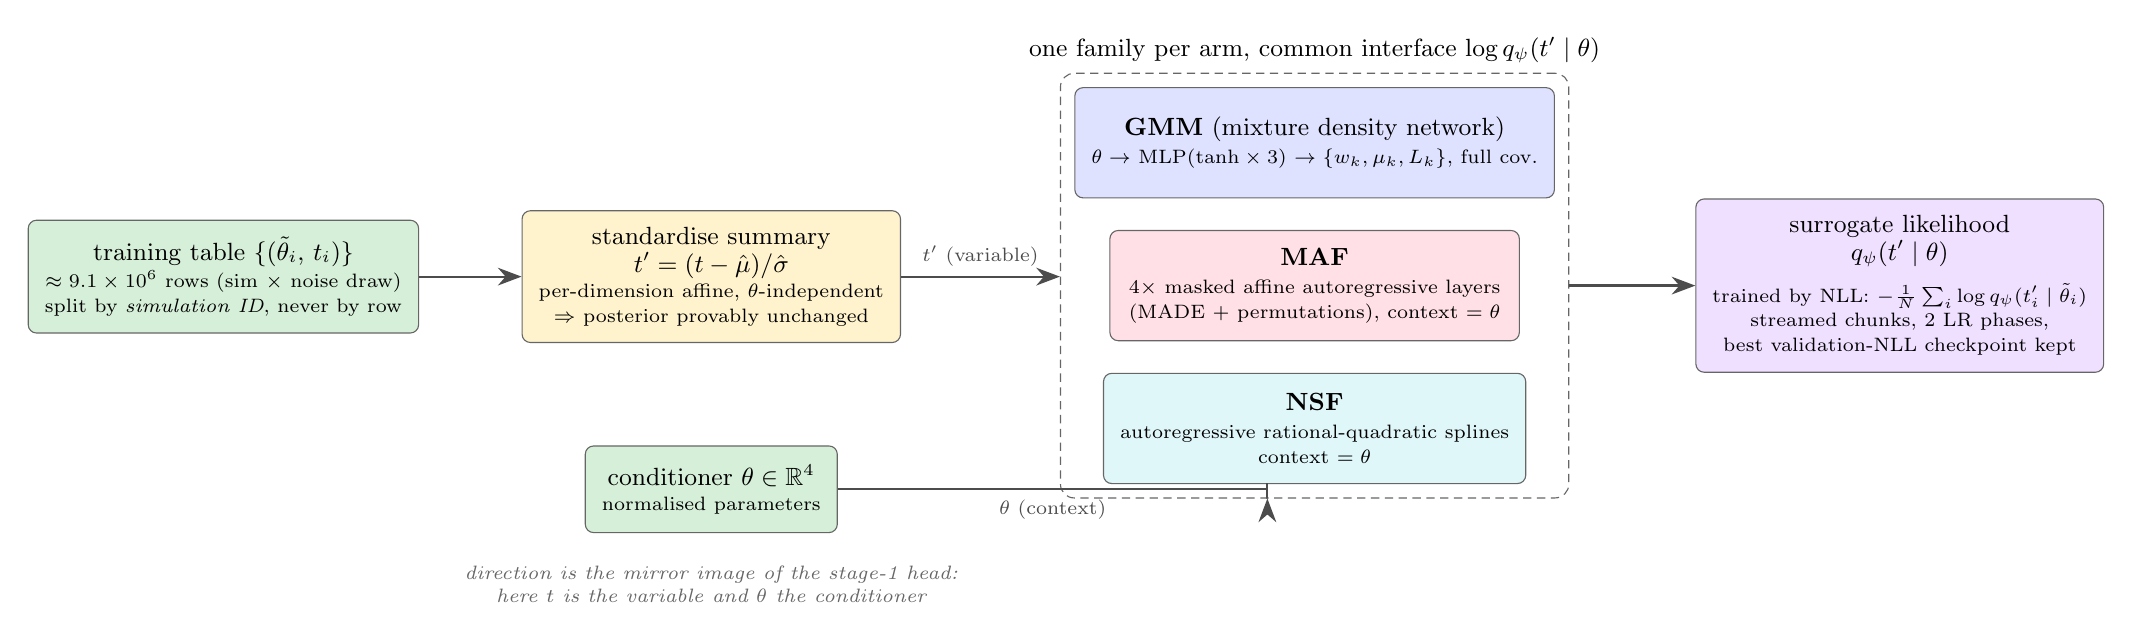
\begin{tikzpicture}[
  node distance=9mm and 13mm,
  every node/.style={font=\small},
  box/.style={draw=black!60, rounded corners=3pt, align=center, inner sep=6pt, minimum height=11mm},
  fam/.style={box, minimum width=52mm, minimum height=14mm},
  arr/.style={-{Stealth[length=3mm]}, thick, black!70},
  darr/.style={arr, densely dashed}
]

% ---------------- inputs ----------------
\node[box, fill=datacol] (table) {training table $\{(\tilde\theta_i,\,t_i)\}$\\[-1pt]
  \scriptsize $\approx 9.1\times10^{6}$ rows (sim $\times$ noise draw)\\[-2pt]
  \scriptsize split by \emph{simulation ID}, never by row};

\node[box, fill=stdcol, right=of table] (std) {standardise summary\\[-1pt]
  $t' = (t-\hat\mu)/\hat\sigma$\\[-2pt]
  \scriptsize per-dimension affine, $\theta$-independent\\[-2pt]
  \scriptsize $\Rightarrow$ posterior provably unchanged};

% ---------------- pluggable estimator families ----------------
\node[fam, fill=gmmcol, right=22mm of std, yshift=17mm] (gmm)
  {\textbf{GMM} (mixture density network)\\[-1pt]
   \scriptsize $\theta \to$ MLP(tanh${}\times3$) $\to \{w_k,\mu_k,L_k\}$, full cov.};
\node[fam, fill=mafcol, below=4mm of gmm] (maf)
  {\textbf{MAF}\\[-1pt]
   \scriptsize $4\times$ masked affine autoregressive layers\\[-2pt]
   \scriptsize (MADE + permutations), context $=\theta$};
\node[fam, fill=nsfcol, below=4mm of maf] (nsf)
  {\textbf{NSF}\\[-1pt]
   \scriptsize autoregressive rational-quadratic splines\\[-2pt]
   \scriptsize context $=\theta$};

\node[draw=black!60, densely dashed, rounded corners=5pt, fit=(gmm)(maf)(nsf),
      inner sep=5pt, label={[font=\small]above:{one family per arm, common interface $\log q_\psi(t'\mid\theta)$}}] (fambox) {};

% theta conditioner
\node[box, fill=datacol, below=13mm of std] (theta)
  {conditioner $\theta\in\mathbb{R}^{4}$\\[-2pt]\scriptsize normalised parameters};

% ---------------- output / training ----------------
\node[box, fill=losscol, right=16mm of fambox] (nll)
  {surrogate likelihood\\[-1pt]
   $q_\psi(t'\mid\theta)$\\[4pt]
   \scriptsize trained by NLL: $-\frac{1}{N}\sum_i \log q_\psi(t_i'\mid\tilde\theta_i)$\\[-2pt]
   \scriptsize streamed chunks, 2 LR phases,\\[-2pt]
   \scriptsize best validation-NLL checkpoint kept};

% ---------------- arrows ----------------
\draw[arr] (table) -- (std);
\draw[arr] (std.east) -- node[above, font=\scriptsize]{$t'$ (variable)} (fambox.west|-std.east);
\draw[arr] (theta.east) -| node[below, font=\scriptsize, pos=0.25]{$\theta$ (context)} ([xshift=-6mm]fambox.south) -- ([xshift=-6mm]fambox.south);
\draw[arr] (fambox) -- (nll);

% note: mirror of stage-1 head
\node[align=center, font=\scriptsize\itshape, text=black!60, below=3mm of theta]
  {direction is the mirror image of the stage-1 head:\\ here $t$ is the variable and $\theta$ the conditioner};

\end{tikzpicture}
\end{document}
